\documentclass{llncs}

\usepackage{graphicx}
\usepackage{url}
\usepackage{booktabs}

% natbib for refs
\usepackage[numbers,sort]{natbib} 

\begin{document}

\title{``{\emph{Come Together!}}'': Interactions of Language Networks and Multilingual Communities on Twitter}

\author{Nabeel Albishry\inst{1}\thanks{This work has been supported by a doctoral research scholarship for
Nabeel Albishry from King Abdulaziz University, Kingdom of Saudi
Arabia.} \and Theo Tryfonas\inst{1} \and Tom
  Crick\inst{2}}

% \thanks{{\emph{N.B.}} The first part of the title of this paper was
% taken from the motto of the 2016 Eurovision Song Contest, which along
% with the theme artwork was said to be ``inspired by the dandelion,
% symbolising the power of resistance and resilience but also of
% regeneration''.}

\institute{Department of Computer Science, University of Bristol, UK\\\email{\{n.albishry,theo.tryfonas\}@bristol.ac.uk}
\and 
Department of Computing, Cardiff Metropolitan University, Cardiff, UK\\\email{tcrick@cardiffmet.ac.uk}}

\maketitle

\begin{abstract}
Emerging tools and methodologies are providing insight into the
factors that promote the propagation of information in online social
networks following significant activities, such as high-profile
international social or societal events; this paper provides insight
into how people are linked, by how different language communities
engage and interact. We present our analysis of a significant online
event and associated interactions in various languages for the 2016
Eurovision Song Contest, that took place on the social networking site
Twitter in May 2016.

By utilising language information from user profiles
({\emph{N}}=1,226,959) and status updates ({\emph{N}}=7,926,746) to
identify and categorise communities, we are able to provide insight
into the pattern of their interactions, as well as constructing their
network graphs to shed light on these multilingual community. The
results show that the nature of the event is reflected on the
engagement degree and wider interaction of communities, as well as
indicating the participation pattern of multilingual users. This
analysis of language communities may also help in deciding which group
of users to engage with -- and hence increase the chance of
influential actions -- when participating in large-scale Twitter
conversations.
\end{abstract}

\section{Introduction}\label{intro}

\subsection{Online Social Networks}
 
In recent years, online social networks have been utilised as
means to express ideas and opinions, share information about events,
or even stimulate and propagate calls for civic engagement and
societal action. Social networking sites such as Twitter, Facebook,
YouTube and Instagram have also empowered individuals to promote their
viewpoints and interests -- professional or otherwise -- to a broad
and diverse global audience. The engagement of certain demographics
with social networks offers the opportunity for researchers interested
in observing and interpreting society to apply established theory and
methods to an emerging digital culture.

To satisfy the demand for various types of communities, interactions
and engagement, there are now vast numbers of specialist and
generalist social media sites and platforms, along with a number of
attempted categorisations. By 2018, there will be an estimated 2.5
billion active social network users (up from 1.9 billion in 2014);
they are producing massive amounts of data (volume) on a real-time
basis (velocity) with implicit sociological attributes such as
beliefs, opinions, sentiments, behaviours, structures and influences
(variety)~\cite{burnap-et-al:2015}. These data exhibit the key traits
of what is referred to as big data: volume, velocity and
variety~\cite{postsm:2014}. In this age of big social data and an
increasingly interconnected digital society, there is a new challenge
-- the application of robust and scalable methods and tools that can
be applied to digitised social behaviour generated via social networks
so as to be able to efficiently analyse these big social data to
provide insight into real-world events and
actions~\cite{lazer-et-al:2009,burnap-et-al:2015}.

Recent
work~\cite{blamey-et-al-2012,schwartz-et-al:2013,blamey-et-al-2013,oatley+crick:2014,oatley-et-al-soccogcomp2015,mostafa-et-al-ai2016}
has analysed what people say and do on social media to identify
distinctive words, phrases, and topics as functions of known
attributes of people such as gender, age, location, or psychological
characteristics. Data can thus be collated and aggregated, inferring
gender, age, location and sentiments, from large-scale social media
data. Potential negative implications of these approaches include the
fact that they can be easily applied to large numbers of people or
groups in society without obtaining their explicit consent or even
being aware it is being done. Data-driven commercial companies,
governmental entities, or even one's followers or friends are able to
use software to infer personality and other attributes -- such as
sexual orientation or political affiliations -- that an individual may
have decided not to share~\cite{lambiotte+kosinski:2014,postsm:2014}.

There are various projects that have used Twitter corpora and related
datasets to make predictions about
elections~\cite{tumasjan-et-al:2010}, stock
markets~\cite{zhang-et-al:2011}, crimes and
policing~\cite{gerber:2014,oatley+crick:2015}, even allowing us to
quantify controversy for topics that spark the most heated debates on
social media~\cite{garimella-et-al:2016}. Twitter played an important
role during what was then known as the ``Arab Spring'', which has been
extensively examined in the social network analysis
domain~\cite{lotan-et-al:2011,howard-et-al:2011,comunello+anzera:2012,wolfsfeld-et-al:2013,bruns-et-al:2013}.
While the use of Twitter data has been demonstrated to provide insight
-- and sociologically relevant demographics~\cite{sloan-et-al:2013} --
into major social and physical events such as
riots~\cite{procter-et-al:2013} and terror
attacks~\cite{burnap-et-al:2014}, often all is not what it may seem;
for instance, many tweets may not a crowd
make~\cite{liang-et-al:2013}.

\subsection{Languages}

Despite the widespread engagement with Twitter globally, little
research has investigated the differences amongst users of various
languages; there is a tendency to assume that the behaviours of
English users generalise to other language
users~\cite{hong-et-al:2011}. Language has featured as a facet of
research on the geographies of Twitter
networks~\cite{takhteyev-et-al:2012}, especially whether offline
geography still matter in online social
networks~\cite{kulshrestha-et-al:2012}. Linguistic-inspired studies
have been done on hashtags~\cite{cunha-et-al:2011}, as well as the
volume and proportional of tweets in English and Arabic, as part of an
analysis of the Arab Spring~\cite{bruns-et-al:2013}. Nevertheless,
language is clearly a vital component of affiliation and discourse on
the web~\cite{zappavigna+martin:2012}, with the creation and curation
of emerging multilingual networks and communities, representing
well-established creative and cultural norms, including for minority
languages such as Welsh~\cite{gj+uj:2013}, as well as investigations
into the economics of linguistic
diversity~\cite{ginsburgh+weber:2011}.

\subsection{Social Network Analysis}

In the social network analysis domain, centrality measures
provide the ability to assess network graphs that are constructed from
collected data (for example, tweets). Selection of these centrality
measures is dependent on the goal of the analysis; for example, the
degree of a node helps to identify nodes with high number of connections
within the
network~\cite{borgatti+everett:2000,rombach-et-al:2014,liu-et-al:2014}.
In a representation of a real-world network, this metric may help to
identify highly connected persons, such as political leaders, sports
stars or celebrities, who are potential ``information
spreaders''~\cite{cha-et-al:2012,borge-holthoefer-et-al:2012,zhang-et-al:2016}.
Centrality measures such as degrees, betweenness, clustering
coefficient, modularity and cliques have been used in many projects to
measure influence or detect the emergence of new
communities~\cite{willis-et-al:2015,oatley+crick:2015}.

Clustering users in communities has been an important analytic factor
in social networking analysis; numerous work has focused on clustering
users based on their locations. However, for the sake of anonymity,
many users tend not to disclose information about their identity, such
as locations~\cite{kang-et-al:2013}. It has also been reported in the
literature that geotagged tweets are generally low in
number~\cite{morstatter-et-al:2013,tan-et-al:2013,kumar-et-al:2014},
the exponential growth in social media over the past decade has been
joined by the rise of location as a central organising
theme~\cite{liang-et-al:2013} of how users engage with online
information services and, more importantly, with each
other~\cite{cheng-et-al:2010,caverlee-et-al:2013}.

\subsection{Overview of Paper}

The remainder of this paper is organised as follows: in
Section~\ref{method} we introduce the methodology and key language
themes.  Section~\ref{eurovisioncasestudy} present the 2016 Eurovision
Song Context case study, along with an analysis of the key data and
results. Section~\ref{conclusions} concludes the paper with a wider
discussion and a summary of the potential application of our approach.


\section{Methodology}\label{method}

The primary purpose of this study is to examine if the nature of event
is reflected in language uses, communities, and diversity on
Twitter. The techniques we introduce in this paper through two
real-world case studies are based on language settings in users'
profiles and those for statuses\footnote{The term `status' is a
generic term used to refer to any Twitter post (tweet, retweet, reply,
or quote).}.  The first step is to identify relationships between
language settings of users and languages used in original posts
(tweets). Then, we will discuss language diversity and how it is
affected by the nature of topic.

\subsection{Users and Locations}

It is important to understand how geotagging works in Twitter. The
`{\emph{place}}' entity included in a Twitter status does not
necessarily indicate precisely where the actual posting was made, as
stated in the Twitter API
documentation\footnote{\url{https://dev.twitter.com/overview/api/places}}:
``{\emph{Tweets associated with places are not necessarily issued from
that location but could also potentially be about that
location}}''. For the sake of anonymity, many users tend not to
disclose information about their identity, particularly locations;
this has also been supported by the literature that geotagged tweets
are generally low in number~\cite{kang-et-al:2013}. We took the step
to verify this claim in our datasets; in the best cases, the ratio of
geotagged tweets did not exceed 2\%.

% In the case of the
% {\texttt{\#BaltimoreRiots}} dataset, only ~1\% of collected statuses
% were associated with places. Moreover, out of this geotagged subset,
% only 4\% were associated with the city where the event took place
% (Baltimore).

An alternative location-based option to consider is based on profile
location, but it still does not serve the need for location clustering
for a multitude of reasons. Firstly, we found that less than 45\% of
users have set their profile location, which is in line with other
studies~\cite{graham-et-al:2014}. Secondly, although Twitter suggests
certain presets for setting profile location, users are given the
option to enter any text they wish; this results in a considerable
amount of noise.

\subsection{Language Communities}\label{langcomm}

Analysis of language communities begins with two basic techniques. The
first is to classify statuses based on their languages, with the
status language extracted from the `{\emph{lang}}' entity inside
status objects. Language used in posting defines which community the
status was meant for; a tweet written in Turkish, for example, is
meant for the Turkish-speaking community. Output from this will be
referred to as `{\emph{posting communities}}'. The second analysis is
to classify users into different communities based on their profile
languages. Output from this technique will be referred to as
`{\emph{profile communities}}'. We can then create network graphs to
explore relationships between profile and posting communities.  As we
will see in the following two case studies, a posting community does
not necessarily indicate the profile community for a user.

\subsection{Language Diversity}\label{diversity}

In this section, we present two language diversity measurements. The
first, which we call `diversity', is to measure uses of languages
different to the profile's i.e. we are referring to `non-selfloop'
edges in the generated network graphs. The second one is to measure
the magnitude of this diversity, which can be calculated as the total
weight of `non-selfloop' over total edge weights in the
profile-posting graph. We will make observation on these two
measurements for both cases.

By observing the language diversity of profile communities, we aim to
measure language diversity of the topic in general. The same technique
can be applied on individual communities within the topic. By doing
so, it can help identify communities that act as bridges between
different profile communities. Moreover, the technique can be applied
to measure diversity at individual users level.


% \section{Case Study: 2015 Baltimore Protests}\label{baltimorecasestudy}

% Following a peaceful funeral that took place on the morning of Monday
% 27 April 2015 in Baltimore, Maryland, USA, a protest hit the
% city. According to the timeline published on the CNN website
% ``{\emph{The city exploded on Monday after the funeral of Freddie
% Gray, a 25-year-old black man who mysteriously died on April 19, a
% week after Baltimore Police arrested
% him.}}''~\cite{baltimorewiki:2015}. The nature of the Baltimore
% protests is a good representation of a partially planned event in
% which a sudden escalation of civil unrest hits a geographical area. The
% event manifested itself on Twitter as {\texttt{\#BaltimoreRiots}}, and
% resulted in more than 1,250,000 status updates.

% Figure~\ref{fig:overallbaltimoreactivity} shows how the event
% manifested itself on Twitter once a ``purge'' was scheduled. We can
% see that what was happening on the ground was quickly reflected in the
% online activity on Twitter. More detailed analysis reveals that within
% one hour the topic started to go ``viral''; more precisely, at
% approximately 15:00 on 27 April at which the ``purge'' was
% scheduled. The topic jumped from roughly 1,200 to 8,000 tweets per
% hour. Then, it peaked with 98,000 between 22:00 and 23:00.

% \begin{figure}[htb]
% \centering
% 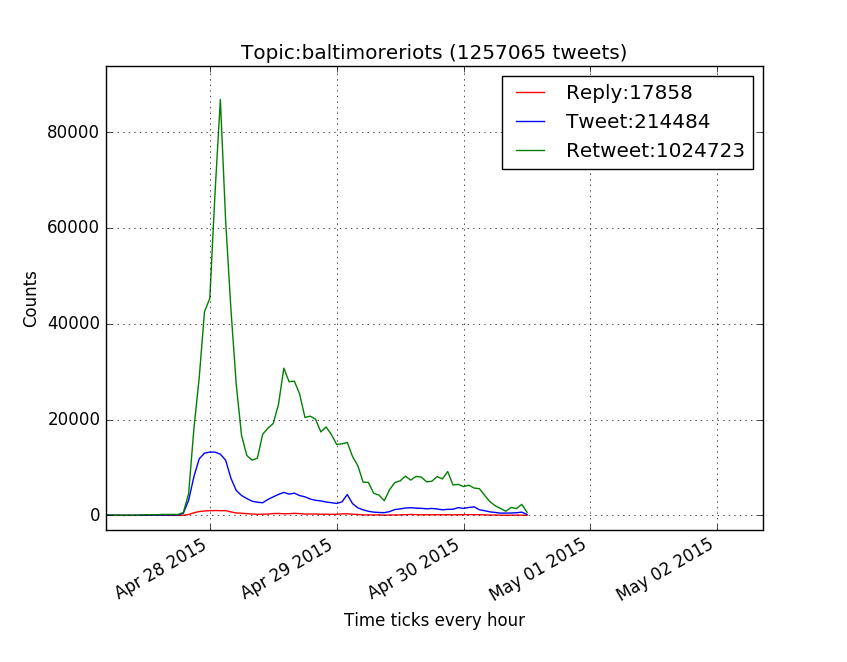
\includegraphics[width=\columnwidth]{images/overallbaltimoreactivity.png}
% \caption{Overall activity for {\texttt{\#BaltimoreRiots}}.}
% \label{fig:overallbaltimoreactivity}
% \end{figure}

% \subsection{Posting Communities}\label{baltimoreposting}

% In the {\texttt{\#BaltimoreRiots}} case, 38 posting languages were
% used for original posts. As we can see in
% Figure~\ref{fig:baltimore_langfreq}, English was the mostly
% frequently-used language by far. Interestingly, results also show that
% language of more than c.7\% statuses could not be identified. When
% investigated, those statuses mostly did not contain text other than
% hashtags, pictures or URLs. Although, this is not a big proportion of
% the overall sample, it came second after English. This category shows
% an interesting case in which qualitative content analysis could
% potentially be used, but it is beyond the scope of this study and will
% not be covered here.

% \begin{figure}[htb]
% \centering
% 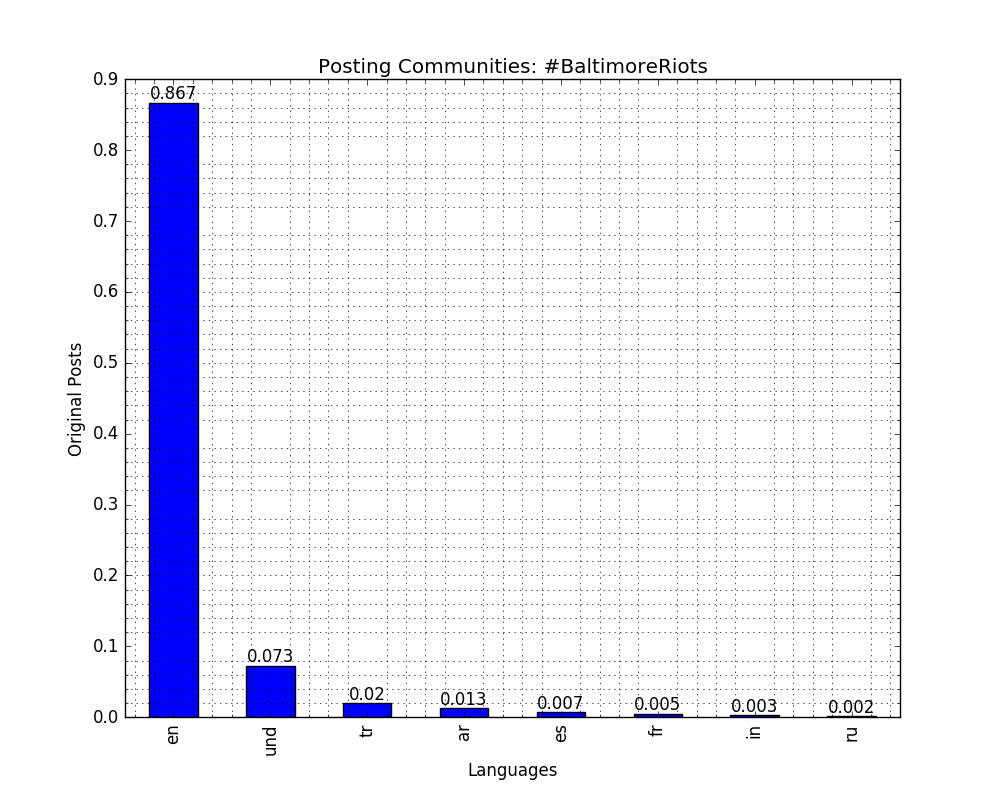
\includegraphics[width=\columnwidth]{images/baltimore_langfreq.png}
% \caption{Most frequently used languages in
%   {\texttt{\#BaltimoreRiots}}: 
% ({\emph{en:}} English; {\emph{es:}} Spanish; {\emph{tr:}} Turkish;
%   {\emph{fr:}} French; {\emph{en-gb:}} British English; {\emph{ar:}}
%   Arabic; {\emph{de:}} German; {\emph{ru:}} Russian; {\emph{it:}}
%   Italian; {\emph{pt:}} Portuguese)}
% \label{fig:baltimore_langfreq}
% \end{figure}

% \subsection{Profile Communities}\label{baltimoreprofile}

% In the majority of cases, users choose to pick a language for their
% Twitter profile settings. In our dataset, we found that out of 716,494
% users, only 45 had not opted to select a language. However, the
% language entity returned by the API for those cases is the initial
% placeholder text ``{\emph{Select Language...}}'' or a translated
% version that may provide hints to the user language
% community. Figure~\ref{fig:baltimore_profile_size} shows that about
% 94\% of the users came from `{\emph{en}}' profile community.

% \begin{figure}[htb]
% \centering
% 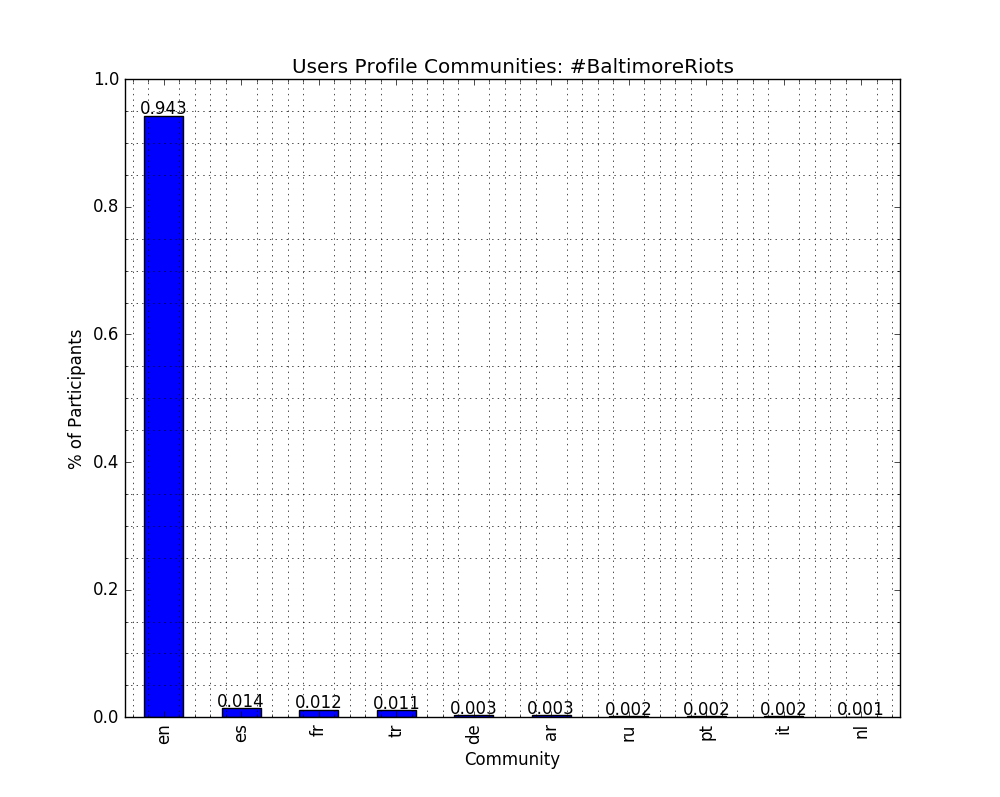
\includegraphics[width=\columnwidth]{images/baltimore_profile_size.png}
% \caption{Top 10 profile language communities in {\texttt{\#BaltimoreRiots}}}
% \label{fig:baltimore_profile_size}
% \end{figure}

% \begin{figure}[htb]
% \centering
% 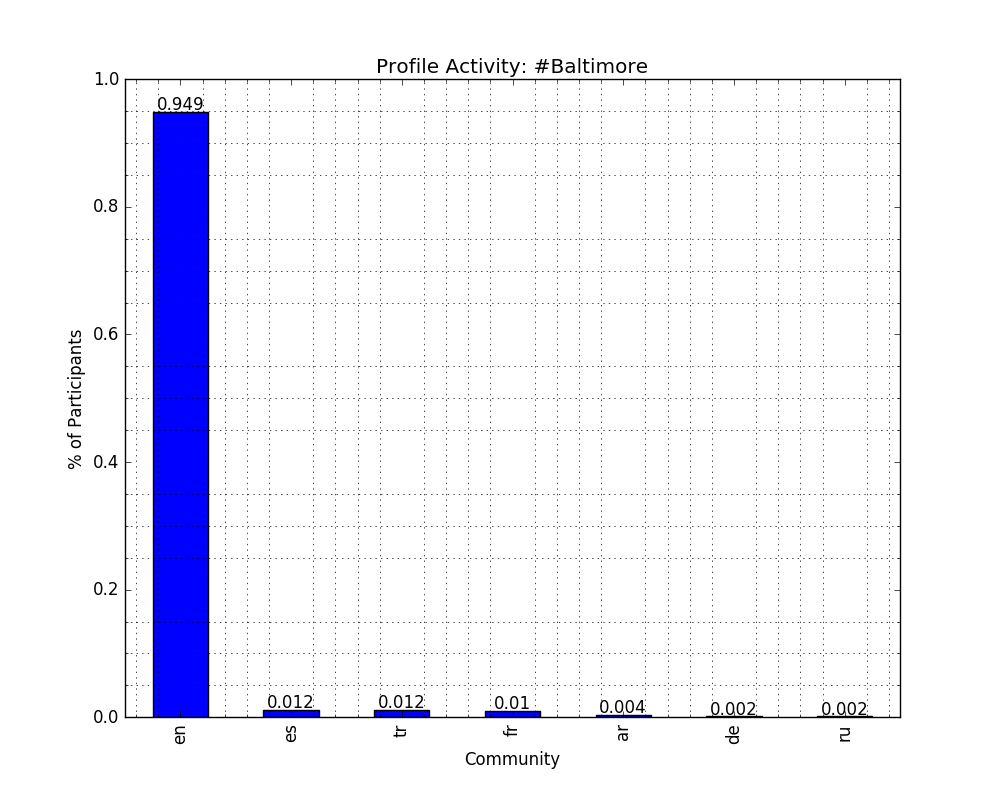
\includegraphics[width=\columnwidth]{images/baltimore_profile_activity.png}
% \caption{Profile language communities causing \%99 of activity in {\texttt{\#BaltimoreRiots}}}
% \label{fig:baltimore_profile_activity}
% \end{figure}

% As we can see in Figure~\ref{fig:baltimore_profile_activity}, activity
% from profile communities is not far from their relative sizes.  Also,
% from these two outputs, we can see that nearly all of the topic
% activity came from one particular community using one particular
% language. This extreme pattern may accompany extreme and
% geographically constrained real-world events such as civil unrest and
% terrorist attacks.

% \subsection{Profile-Posting Network}

% This section explores the network graph we are able to build from
% profile-posting relationships; constructing this graph is an essential
% step for our core analysis of language diversity. For example, to
% investigate whether the `{\emph{en}}' posting community is linked to
% particular profile communities, we used the bipartite graph as
% presented in figure~\ref{fig:baltimore_p_s_lang_sl}.  In this graph,
% nodes that are prefixed by ``{\emph{p\_}}'' represent profile language
% community, and nodes that are prefixed by ``{\emph{s\_}}'' represent
% posting language community. The size of node represents the weighted
% indegree, whereas colour represents the outdegree: the darker the
% colour, the higher outdegree; hence, completely white nodes have no
% outdegree and help to easily distinguish posting communities from
% profile ones. From the graph we can infer that there is a dominating
% player in both domains: posting languages and profile communities.
% Therefore, for the case of {\texttt{\#BaltimoreRiots}}, we can
% conclude that the case was substantially localised.

% \begin{figure*}[!htb]
% \centering
% 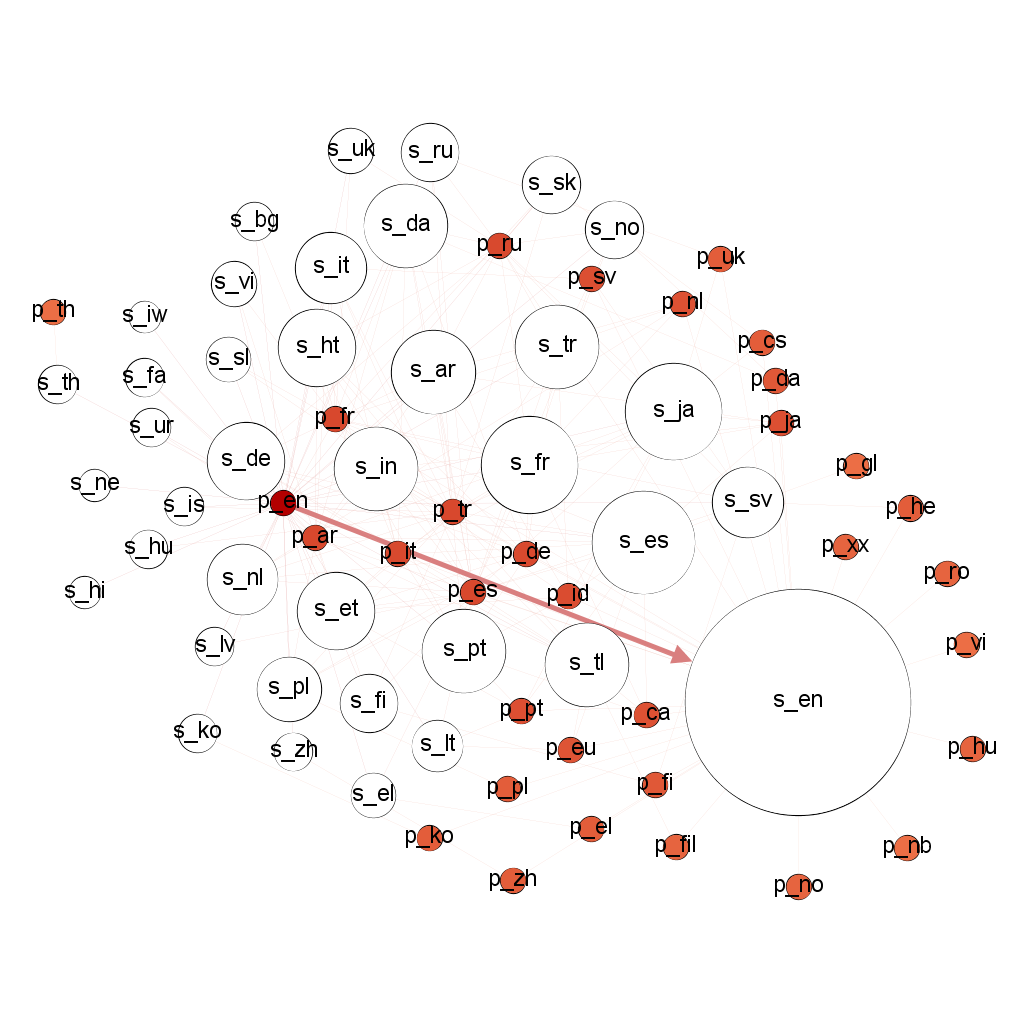
\includegraphics[width=0.8\textwidth]{images/baltimore_p_s_lang_sl.png}
% \caption{Profile-posting network graph}
% \label{fig:baltimore_p_s_lang_sl}
% \end{figure*}


% \subsection{Diversity and Multilingual Communities}

% To examine users' behaviour in using languages other than their own
% (profile language), same-language communities are filtered out.  We
% found that English profile users frequently posted in Arabic, as a
% secondary posting language. This sort of activity could be obtained
% from edge weights in the profile-posting
% graph. Table~\ref{tbl:baltimoredifflang} shows the top portion of
% these communities. This observation sheds light on those
% relationships, and could be of use for further analysis, such as
% identifying highly disseminated message that fall into these
% relationships and their contents.

% \begin{table}[!htb]
% \centering
% \begin{tabular}{@{}lcr@{}}
% \toprule
% \textbf{Profile-Posting Edge} & \textbf{Weight} \\ \midrule
% {\emph{en-ar}} & 1.00 \\
% {\emph{es-en}} & 0.49 \\
% {\emph{ar-en}} & 0.47\\ 
% {\emph{fr-en}} & 0.38 \\
% {\emph{tr-en}} & 0.37 \\
% {\emph{en-tr}} & 0.36 \\ \bottomrule
% \end{tabular}
% \caption{Users' behaviour in using languages different to their profile (normalised)}
% \label{tbl:baltimoredifflang}
% \end{table}

% The topic diversity in {\texttt{\#BaltimoreRiots}} is 0.91, which is
% not surprising when we recall that there were 38 languages used in
% original tweets. However, when the magnitude of diversity was
% measured, it gave a score of 0.04, a generally low score. This will be
% of use when compared to the data from our second case study in Section
% ~\ref{eurovisioncasestudy}.

% Additionally, measuring multilingual communities is another use of
% profile-posting network graph at individual users' level. We grouped
% users based on their relationship with posting communities, regardless
% of their profile language. For example, a user posting in both
% `{\emph{en}}' and `{\emph{fr}}' will be classified as bilingual, and
% so on. Based on this grouping technique, with the `{\emph{und}}' lang
% category eliminated, we identified nine sets. As we can see in
% Figure~\ref{fig:baltimore_multilingual}, monolingual group contain the
% overwhelming majority of users (nearly 99\%), contributing
% approximately 94\% of the topic activity too.

% \begin{figure}
% \centering
% 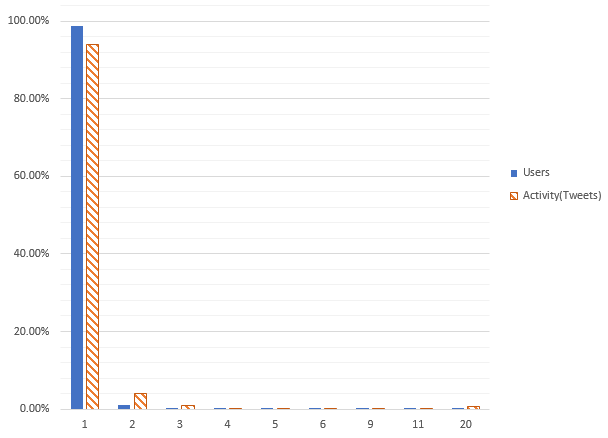
\includegraphics[width=\columnwidth]{images/baltimore_multilingual.png}
% \caption{Multilingual communities and their activity in {\texttt{\#BaltimoreRiots}}}
% \label{fig:baltimore_multilingual}
% \end{figure}


\section{Case Study: 2016 Eurovision Song Contest}\label{eurovisioncasestudy}

The Eurovision Song Contest is the longest-running annual
international TV song competition, held, primarily, among the member
countries of the European Broadcasting Union since 1956. Each
participating country submits an original song to be performed on live
television and radio and then casts votes for the other countries'
songs to determine the most popular song in the competition. The
contest has been broadcast every year for sixty years, and is one of
the longest-running television programmes in the world. It is also one
of the most watched non-sporting events in the world, with audience
figures varying in recent years from 100 million to 600 million
globally\footnote{\url{https://www.eurovision.tv}}. The emergence of
social networking in recent years has dramatically changed the range
and scope of audience interaction and engagement, particularly for
different language communities.

The 2016 Eurovision Song
Contest\footnote{\url{https://www.eurovision.tv/page/stockholm-2016/all-participants}}
took place in May in Stockholm, Sweden. There were 32 countries taking
part, with two semi-finals taking place on 12 and 14 May, with 26
countries qualifying for the final on 16 May. This year's contest was
perceived by many commentators to be tense and politically motivated,
especially with Ukraine eventually winning the
final~\cite{telegrapheuroboycott:2016}. Varying analyses see the
contest as being influenced by political conflicts, friendships or
cultural
bias~\cite{ginsburgh+noury:2008,charron:2013,blangiardo+baio:2014,budzinski+pannicke:2016},
with a range of news articles explicitly discussing the possibly
biased results~\cite{telegrapheurobias:2016}.  Twitter activity was
very high throughout the event on the primary {\texttt{\#Eurovision}}
hashtag. The participation exceeded 7,900,000 statuses, produced by
1,226,959 users; Figure~\ref{fig:overalleurovisionactivity} shows the
overall Twitter activity.

\begin{figure}[htb]
\centering
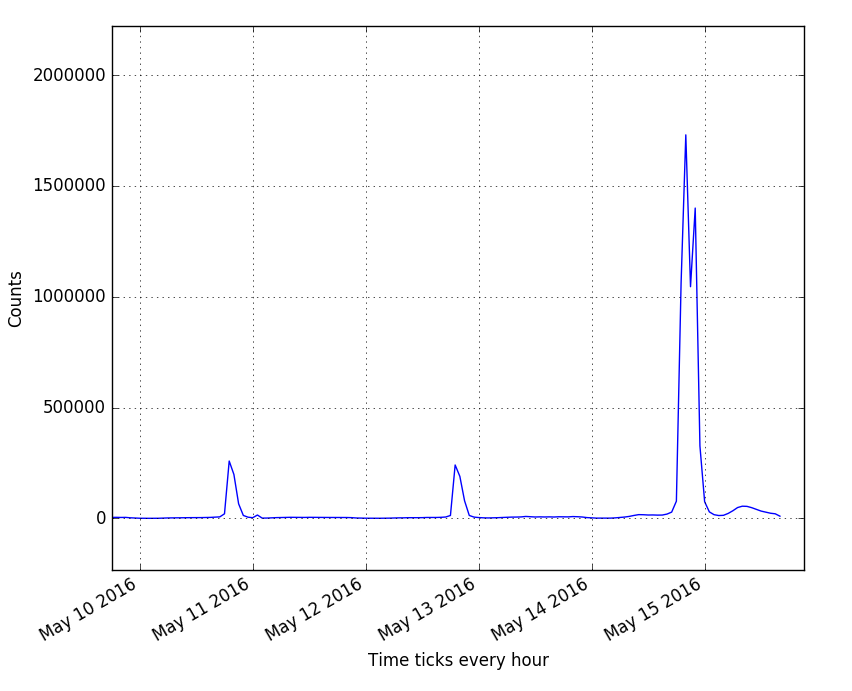
\includegraphics[width=\columnwidth]{images/overalleurovisionactivity.png}
\caption{Overall activity for {\texttt{\#Eurovision}}.}
\label{fig:overalleurovisionactivity}
\end{figure}

Preliminary analysis shows that tweets and retweets together account
for 97\% from the total activity; these two subsets can be
representative on their own, without the need to include other
interaction sets, such as replies and quoted tweets. It is important
to note that tweets and retweets are used to measure actions, and
reactions, respectively. However, our analysis will be focusing on
original tweets only and the usage of different languages in this set.

\subsection{Posting Communities}\label{eurovisionpostingcomm}

In the {\texttt{\#Eurovision}} case, there were 49 posting
languages. Fig~\ref{fig:eurovisionlangfreq} shows the top posting
languages (tweets), out of 3,834,937. As might be expected, English
was the most frequently-used posting language, while c.4\% statuses
could not be categorised. However, as we can see, it is not as
dominating as in the {\texttt{\#Baltimoreriots}} case. Interestingly,
it took participation from eight posting communities to match the
activity ratio of the `{\emph{en}}' posting community in
{\texttt{\#Baltimoreriots}} (~0.87).

\begin{figure}[htb]
\centering
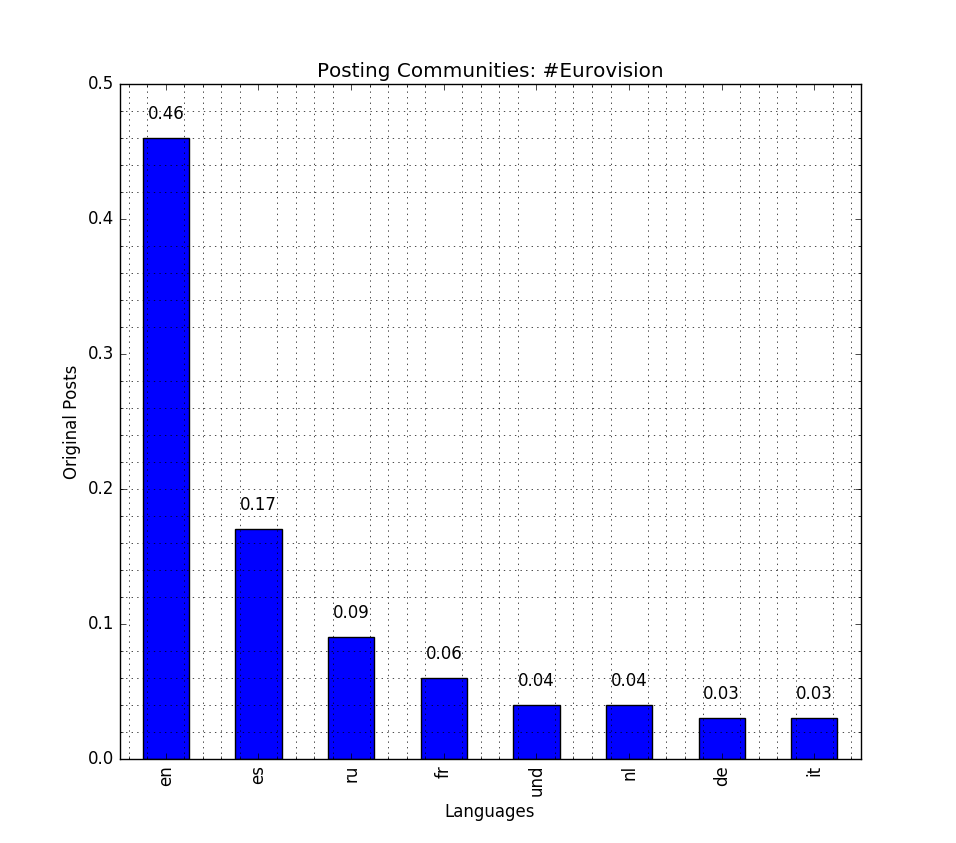
\includegraphics[width=\columnwidth]{images/eurovision_langfreq.png}
\caption{Most frequently used languages in {\texttt{\#Eurovision}}.}
\label{fig:eurovisionlangfreq}
\end{figure}

\subsection{Profile Communities}\label{ppcomm}

In total, 1,226,959 users interacted with the {\texttt{\#Eurovision}}
hashtag. In terms of their profile languages, they formed 50
communities. Figure~\ref{fig:eurovisionprofilesize} shows some of the
top profile communities from of all users, ordered by size. Unlike
status language, profile language relies on the user to pick a
language for their Twitter profile settings. In general, the default
value of this option is the initial placeholder text ``{\emph{Select
Language...}}'' or a translated version that might provide hints
regarding the user language community. In {\texttt{\#Eurovision}}
dataset, we found that all users had selected a language and no users
with the default value.  For completeness, we also show profile
communities grouped by their activity in
~\ref{fig:eurovisionprofileactivity}.

\begin{figure}[htb]
\centering
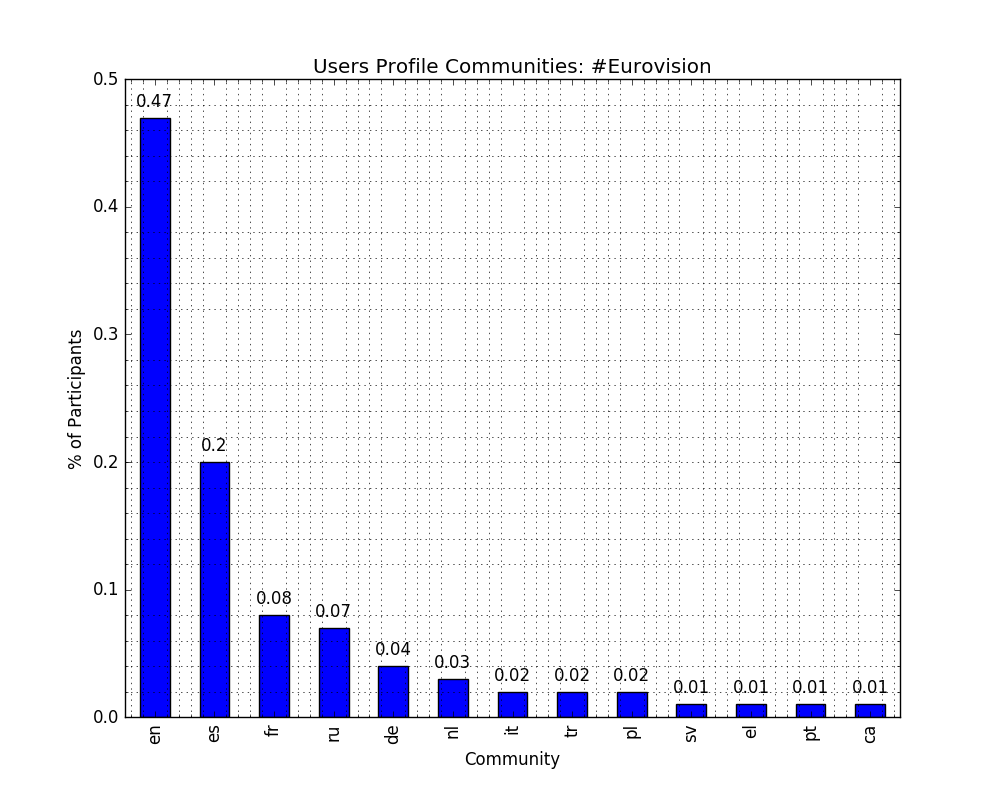
\includegraphics[width=\columnwidth]{images/eurovision_profile_size.png}
\caption{Profile communities by size in {\texttt{\#Eurovision}}.}
\label{fig:eurovisionprofilesize}
\end{figure}

\begin{figure}[htb]
\centering
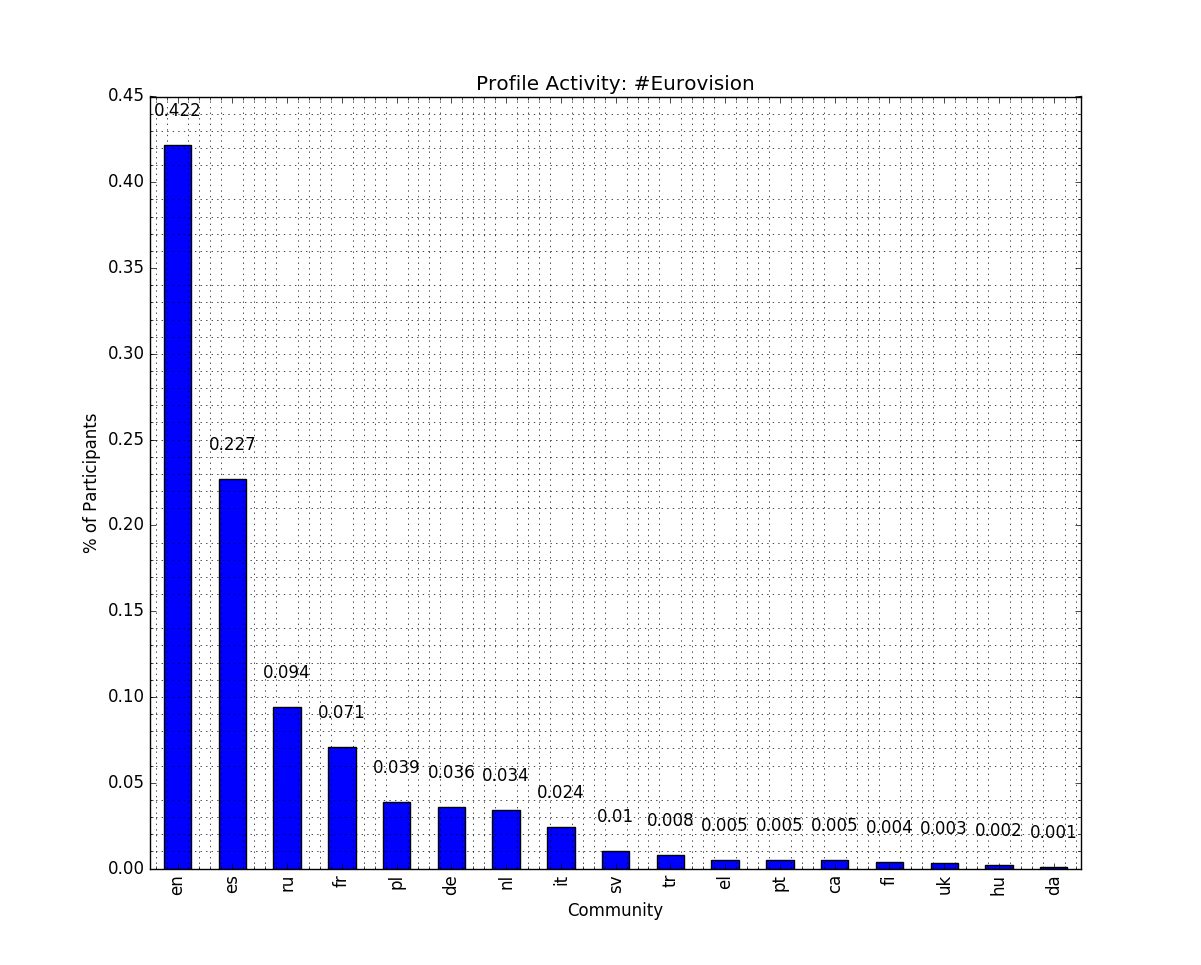
\includegraphics[width=\columnwidth]{images/eurovision_profile_activity.png}
\caption{Profile communities by activity in {\texttt{\#Eurovision}}.}
\label{fig:eurovisionprofileactivity}
\end{figure}

From the previous three figures, we can see clear similarities between
the posting and profile communities. Statistically, we found that
these three measures (i.e. profile community size, profile activity,
and frequency of language uses) are highly correlated, for both case
studies. An interesting example to explore here is the comparison
between two profile communities, `{\emph{fr}' and `{\emph{ru}}' .  We
can see that although the French community had more presence, the
Russian posting community is greater. A simple explanation would be
that the Russian profile community was relatively more active than
French due to the focus on related countries; another reason could be
the participation of non-Russian profiles using the Russian language
for posting; further discussion of this example follows in the next
section.

\begin{figure*}[!htb]
\centering
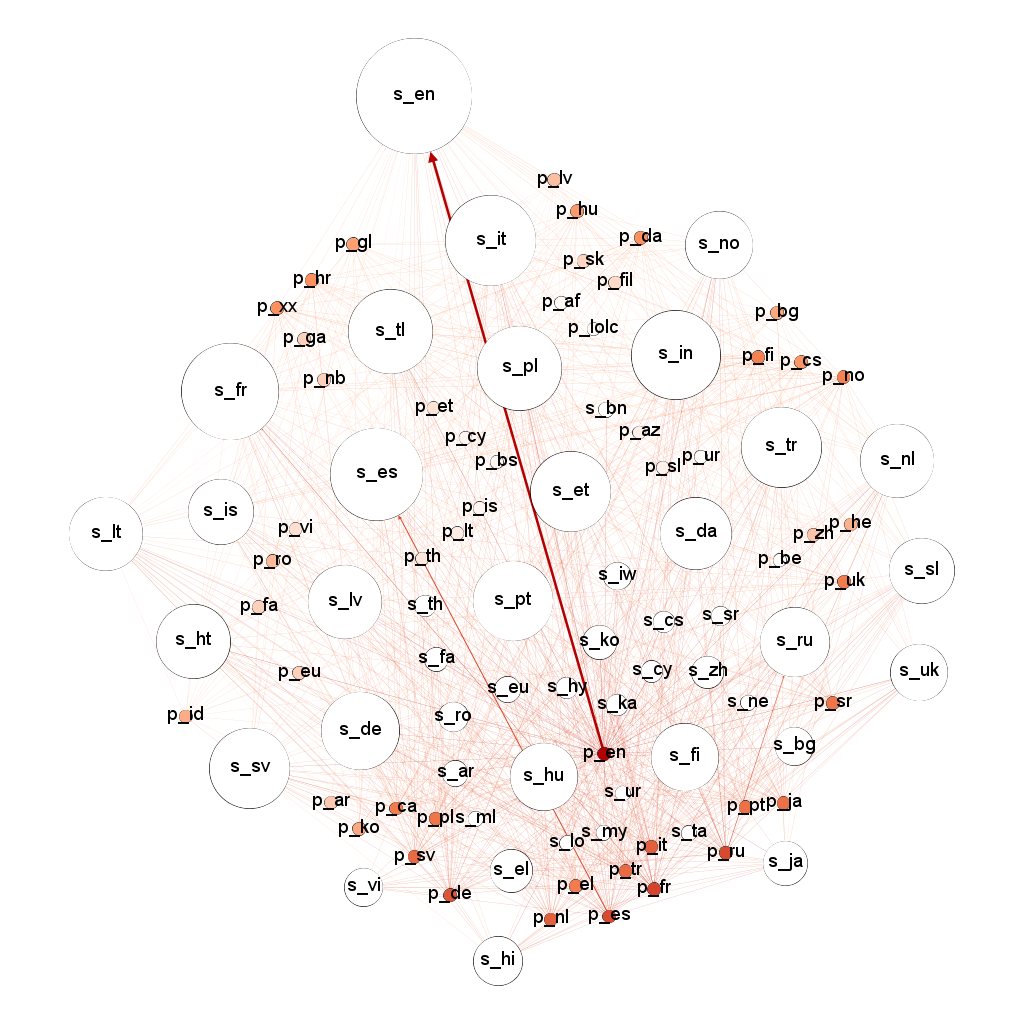
\includegraphics[width=0.8\textwidth]{images/euro_pslang.png}
\caption{Profile-posting network graph for {\texttt{\#Eurovision}}}
\label{fig:eurovisionpslang}
\end{figure*}

\subsection{Profile-Posting Analysis}\label{eurovisionppanalysis}

To explore the posting behaviour from profile communities, we
constructed the graph shown in Figure~\ref{fig:eurovisionpslang},
allowing us to continue analysing the '{\emph{fr}}' and '{\emph{ru}}'
example.  The graph helps us to evaluate contributions of profile
communities to the Russian posting community, with Russian language
profile communities resulted in more than 95\% of activity in this
posting community. The relative weights from those profile communities
to the Russian posting community were {\emph{ru}}: 91.25\% and
{\emph{en}}: 7.26\%.

% \begin{table}[!htb]
% \centering
% \begin{tabular}{@{}lc}
% \toprule
% \textbf{Community} & \textbf{\%} \\ 
% \midrule
% {\emph{ru}} & 91.25 \\
% {\emph{en}} & 7.26 \\
% \bottomrule
% \end{tabular}
% \caption{Active profile communities within the Russian posting community}
% \label{tbl:russian}
% \end{table}

However, posts in Russian were not just appearing from the Russian profile
community. This show one way of exploring relationships between
profile and posting communities, especially if we are interested in
particular communities. Another approach is to explore the posting
behaviour of one particular community. When considering certain
profile communities, there is a tendency to assume that communities
only post in languages that are the same as their profile language. To
examine this assumption, we investigated participation of
`{\emph{en}}' profiles, as they form nearly 50\% of users. In total,
there were 1,841,205 posts from this community, 81\% of which were
posted in `{\emph{en}}', 15.4\% in other languages, and 3.62\% were
not identified. Table~\ref{tbl:enpartlangs} lists the top 95\% posting
languages used by this profile community.

\begin{table}[!htb]
\centering
\begin{tabular}{@{}lc}
\toprule
\textbf{Language} & \textbf{\%} \\ 
\midrule
{\emph{en}} & 80.99 \\
{\emph{und}} & 3.62 \\
{\emph{es}} & 2.69 \\
{\emph{nl}} & 2.39 \\
{\emph{fr}} & 1.39 \\
{\emph{ru}} & 1.36 \\
{\emph{de}} & 0.97 \\
{\emph{it}} & 0.87 \\ 
{\emph{el}} & 0.86 \\ 
\bottomrule
\end{tabular}
\caption{Top 95\% of participation languages from `{\emph{en}}' profiles}
\label{tbl:enpartlangs}
\end{table}

\subsection{Diversity and Multilingual Communities}

All of the 49 profile communities have used different languages in
posting. 16 out of those communities did not use their own language,
although they were low in numbers of tweets and engagement. Moreover,
in terms of using different languages, we found that 32 communities
scored at least 50\% out of their original tweets.

We also wanted to measure the diversity and its magnitude for the
topic.  We found that the language diversity of the topic as a whole
is 0.96. Although the diversity here is not far from
{\texttt{\#BaltimoreRiots}} case, when we compare magnitude of
diversities, it scored 0.22, which is relatively high.

In terms of multilingual communities, we group users based on their
relationship with posting communities, as we did in the
{\texttt{\#BaltimoreRiots}} case.  Based on this grouping technique,
with the `{\emph{und}}' lang category eliminated, we identified 20
sets. The smallest two groups consist of one user each, who posted in
22 and 25 different languages.  As we can see in
Figure~\ref{fig:multilingual}, monolingual users scored about 85\% of
all users, creating 47\% of the total original posts. Although we
cannot conclude that there is a correlation between high
multilingualism and illegitimacy of accounts, this would be an
interesting further topic to investigate.

\begin{figure}[htb]
\centering
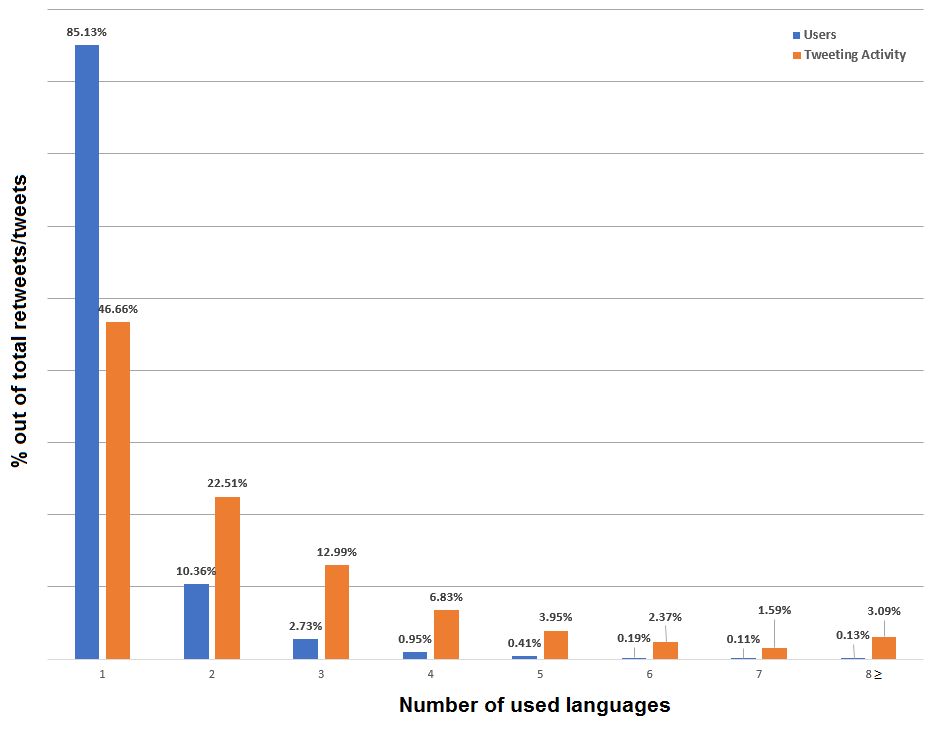
\includegraphics[width=\columnwidth]{images/multilingualcommunities.png}
\caption{Multilingual communities and their associated activities.}
\label{fig:multilingual}
\end{figure}


\section{Conclusions}\label{conclusions}

This paper presents work in identifying language interactions within
multilingual communities using a high-profile real-world case study --
the 2016 Eurovision Song Contest -- and the associated engagement and
interactions on Twitter. As we discussed in Section~\ref{langcomm},
the nature of the event (e.g. being a local or global) may be
reflected on community conversations on Twitter. We found that the
majority of posting activity comes from the main community (the
language community in which the incident has happened or closely
related). This is especially true when the online conversations are
triggered by a real-world incident. The same is the case for posting
languages -- users mostly use the language of the main
community. Furthermore, there is a positive relationship between size
of profile and posting communities; we have also demonstrated that a
large number of people in participating profile communities does not
necessarily imply high language diversity, as single posts from many
profile communities are enough to dramatically affect the diversity of
the topic. We also presented the diversity magnitude measurement, and
showed that it is highly effective in eliminating, or at least
minimising, the noise caused by those odd posts.  We also discussed
the structure of multilingual communities and their activity.  In a
few cases, users may use a significant number of languages, up to 25
different languages. These extreme cases may be interesting to
investigate for possible spammer/false account detection or for
sociolinguistics in more moderate cases.

We also presented a network graphs showing how language communities
relate to each other, as well as relations between profile and posting
communities. We find that this second graph is important to facilitate
comparing users' defined profile language with their posting
language. Some events might be termed as `partially scheduled' as
their end was different to how they were planned in the first place;
in such situations, we noticed that there always be a dominating
community and language.

The methods we have presented here can be used in identifying how
communities interact with one another, which ones are most active,
which languages are mostly used, and at what time. Applying these
techniques on data pouring from the Twitter Stream
API\footnote{\url{https://dev.twitter.com/streaming/overview}} would
be applicable to a wide number of domains. For example, these methods
can be used in social network marketing and publicity to increase the
probability of influential posts. In practice, for a given
{\texttt{\#<Brand>}}, by monitoring the activity of different language
community, one can decide the time to post well-tailored tweets
targeting certain communities.

Moreover, within certain contexts, the order of applying these two
classifications (posting and profile) will generate different results.
For example, taking one profile community and dividing it into
different posting communities shows the number of languages this
community may use, and hence degree of openness and reachability. A
possible scenario for governments, politicians or campaigners would be
to use this method to measure to what extent other languages are used
within a profile community. It may also show how users associate
themselves with one community in their profile while using other
languages. Monitoring unusual activity for secondary languages may
help to uncover important messages or opinions that could not be
openly expressed, for a variety of reasons, to the rest of the profile
community. For the social network analysis domain, this method
provides a different perspective for influence analysis. Endorsement
from different profile communities cannot be measured similar to those
coming from the same community.

As we saw in the comparison between the two case studies, we can
conclude that the nature of the event is mostly reflected on the
``language diversity magnitude'' than any other measurement.  For
future work, we will explore in more detail how multilingual
communities interact and participate, as well as their reaction
networks. We believe that differentiating between endorsements
(e.g. retweets) and other reactions may provide further insight into
the networks and communities. Furthermore, we will apply the methods
presented in this paper on other high-profile event/discussion
datasets in different domains or contexts, such as for sports, music
contests and civil rights/humanitarian actions, to provide further
insight into the methodology and overall approach.

% \begin{acks}
% This work has been supported by a doctoral research scholarship for
% Nabeel Albishry from King Abdulaziz University, Kingdom of Saudi
% Arabia.
% \end{acks}


% bib
\bibliographystyle{abbrvnat}
\bibliography{icci2017}

\end{document}
